\documentclass[13pt]{article}
\renewcommand{\baselinestretch}{1.0}
\usepackage[utf8]{vietnam}
\usepackage[a4paper, total={6in, 8in}]{geometry}
\usepackage[vietnamese,english]{babel}
\usepackage{hyperref}
\usepackage{mathtools}
\usepackage{amssymb}
\usepackage{indentfirst}
\usepackage{graphicx}
\usepackage{minted}
\usepackage{ragged2e}
\usepackage[nottoc]{tocbibind}

\hypersetup{
    colorlinks=true,
    linkcolor=blue,
    citecolor=blue,
    urlcolor=blue,
}
\begin{document}
\begin{titlepage}
    \begin{center}
        \vspace*{1.8cm}
        \Large
        Distributed System Labwork 3\\
        \Large
        \vspace{0.5cm}
        \begin{center}
            
\includegraphics[scale=1.0]{logo USTH-01.PNG}
        \end{center}  
        \vspace{0.5cm}
            Group 6 - ICT\\
        \vspace{0.5cm}
            University of Science and Technology of Hanoi\\
        \vspace{0.5cm}
            February, 2022
        \vfill
          
   \end{center}
\end{titlepage}

\newpage
\tableofcontents
\newpage

\section{Introduction}
\subsection{Overview}
\noindent%
MPI (Message Passing Interface) is a library that allows users to write programs that can run on most parallel architectures effectively. The processes working in parallel have independent address spaces in the message-passing paradigm of parallel computing. When a piece of one process's address space gets copied into the address space of another process, communication happens. This is a cooperative operation that occurs only when the first process sends data and the second process receives data.

\noindent%
In this labwork, we try to build a file transfer system using MPI. We will use Python in this labwork.

\subsection{Protocol}

\begin{figure}[h]
    \centering
    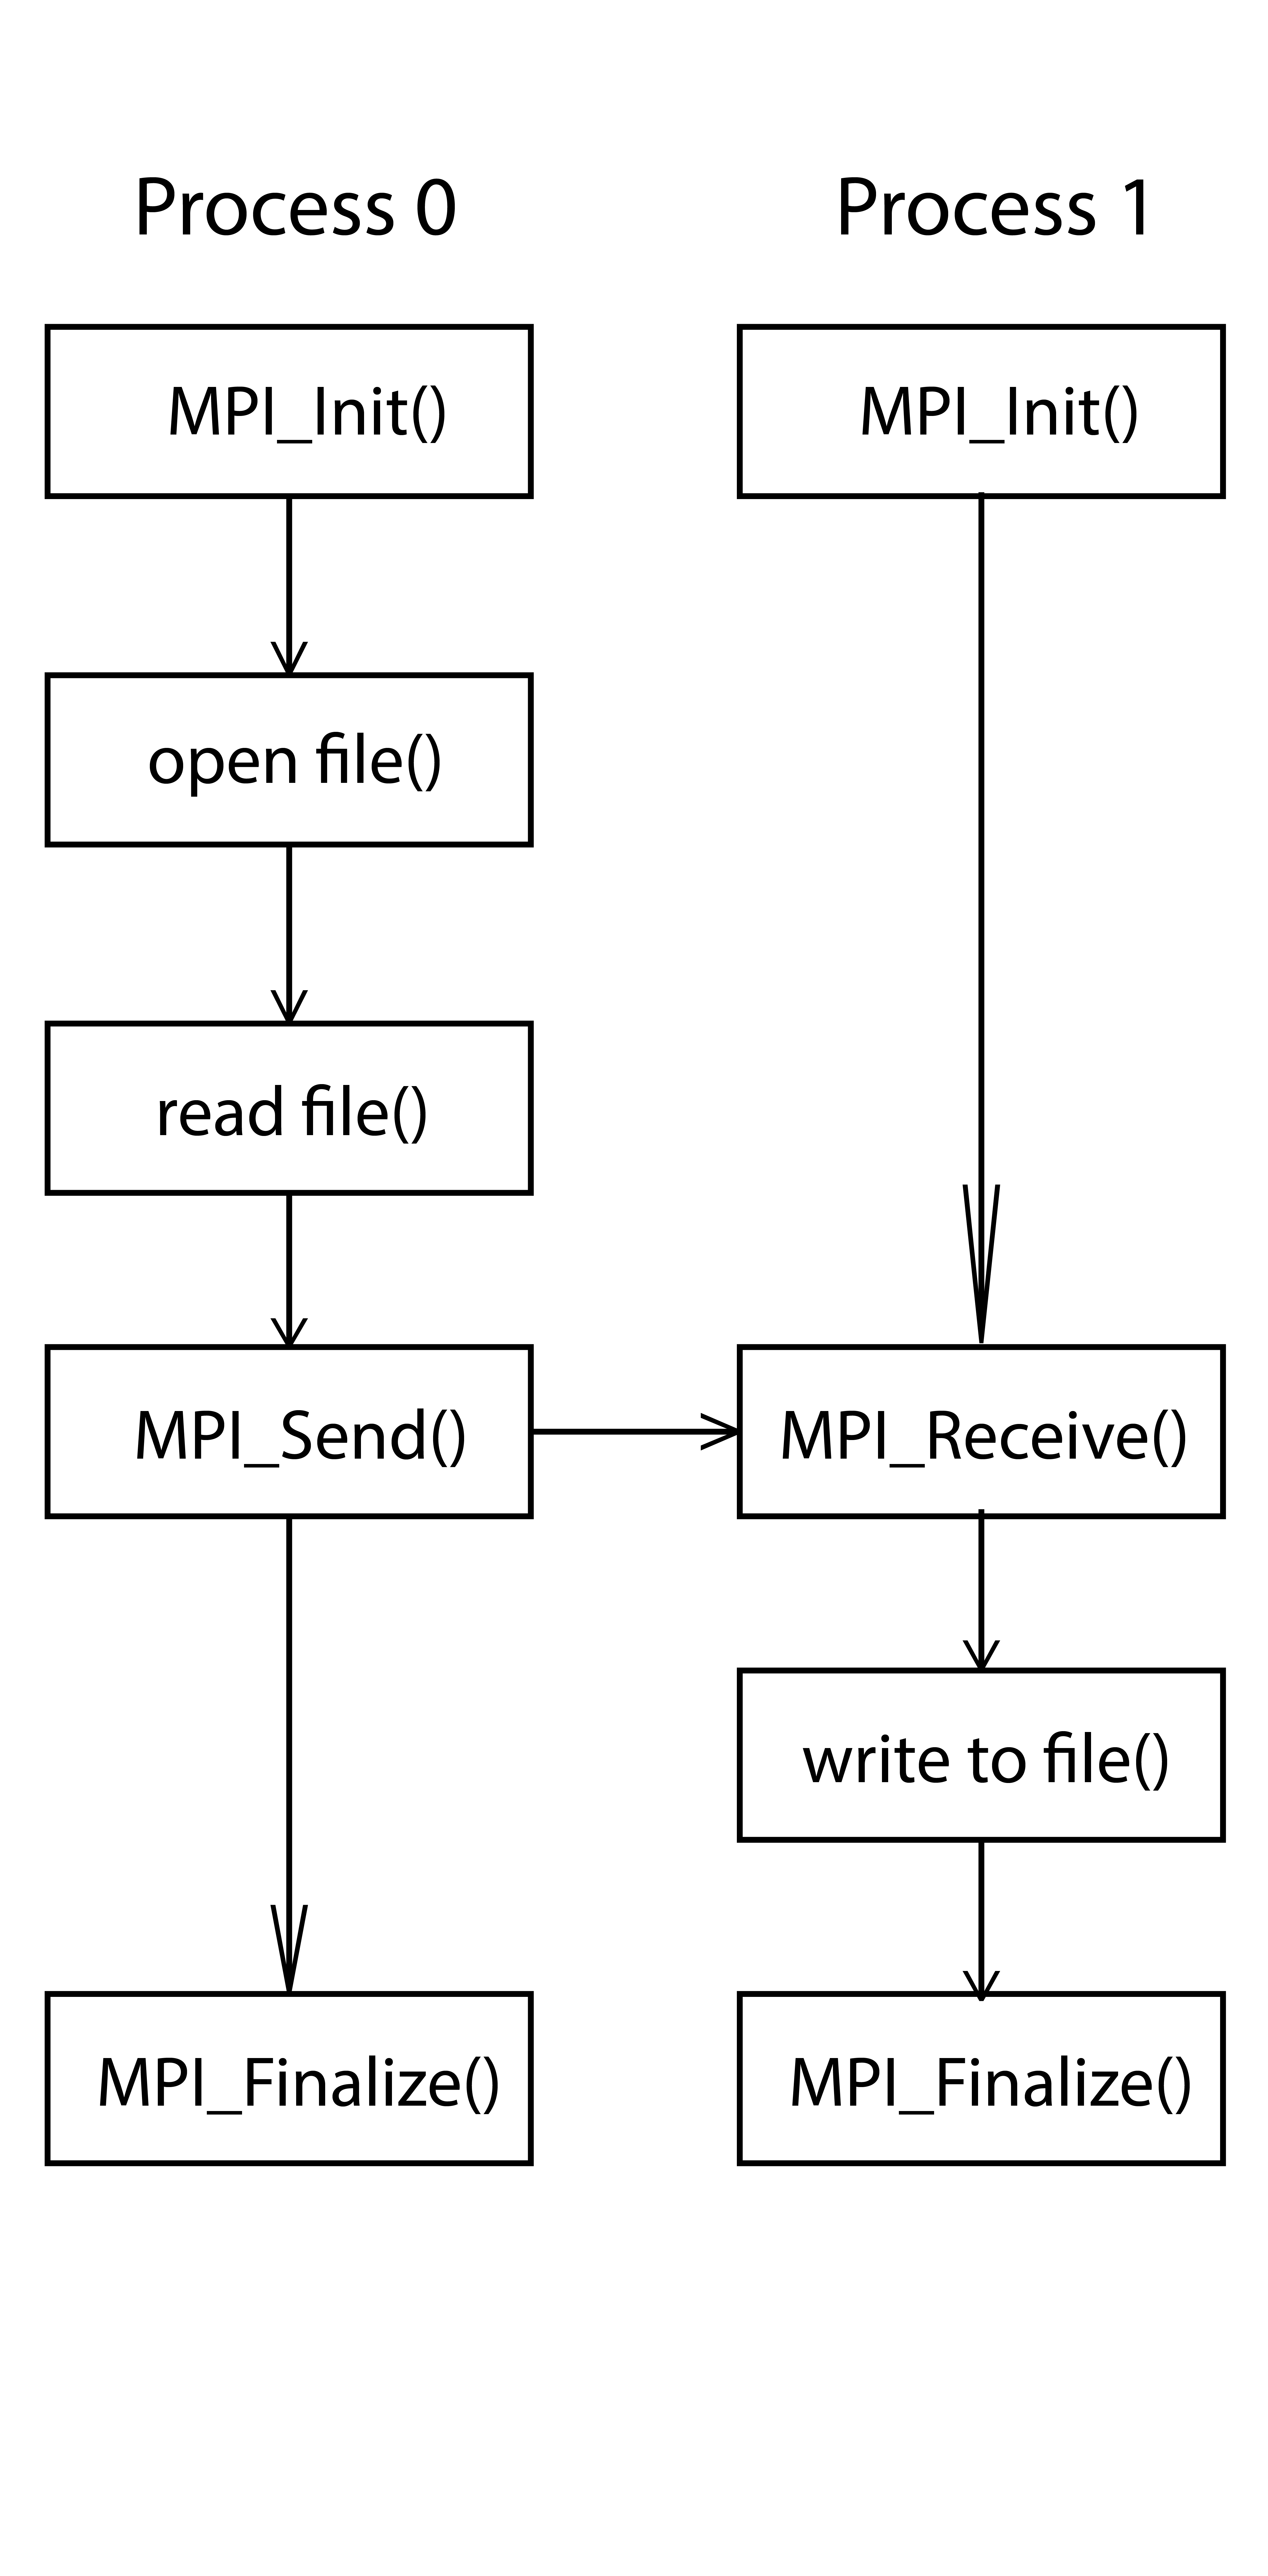
\includegraphics[scale=0.1]{protocol-diagram-01.png}
    \caption{Protocol diagram}
    \label{fig:protocol}
\end{figure}



\subsection{Implementation}
\noindent%
This is the implementation of the labwork

\noindent
To run the program, please type "mpiexec -n 2 python mpi.py"

\begin{minted}{python}
# To run this program
# Install MPI from Microsoft
# Check install successfully in terminal: mpiexec
# Run this program: mpiexec -n 2 python mpi.py
# Done
from mpi4py import MPI
import os

comm = MPI.COMM_WORLD
size = comm.Get_size()
rank = comm.Get_rank()

fileName = os.path.basename("./filetransfer.txt")
fileContent = open("filetransfer.txt", "r").read()

sentMail = (fileName, fileContent)

if rank == 0:
  comm.send(sentMail, dest=1)
  print("From rank", str(rank), "we sent: ", sentMail)
  
if rank == 1:
  receivedMail = comm.recv(source=0)
  print("From rank", str(rank), "we received: ", receivedMail)
  f = open("./mailbox/" + fileName, "w")
  f.write(receivedMail[1])
  f.close()
  print("Check mail in mailbox!")
\end{minted}

\subsection{Contribution}
\noindent%
\begin{table}[ht!]
  \begin{center}
    \label{tab:table1}
    \begin{tabular}{l|l}
      \textbf{Member} & \textbf{Contribution}\\
      \hline
      Nguyen Quang Vinh & Send fIle code\\
      Nguyen Tran Nguyen & Receive file code\\
      Mai Xuan Hieu & Design Protocol\\
      Nguyen Anh Quan & MPI concept\\
      Nguyen Tuong Quynh & Report\\
    \end{tabular}
    \caption{Contribution Table}
  \end{center}
\end{table}
\end{document}